\documentclass{article}
\usepackage{amsmath}
\usepackage[margin=1.5in]{geometry}
\usepackage{graphicx}
\usepackage{listings}
\usepackage[T1]{fontenc}
\usepackage[utf8]{inputenc} % Added for Polish characters in source
\usepackage[polish,english]{babel} % Added for Polish hyphenation and terms if needed
\usepackage{float}
\usepackage{circuitikz}
\usepackage{xcolor} % Added for color definitions in lstlisting

\lstdefinestyle{Solidity}{
  language=Solidity,
  basicstyle=\ttfamily\small,
  keywordstyle=\color{blue},
  commentstyle=\color{green!40!black},
  stringstyle=\color{red},
  numbers=left,
  numberstyle=\tiny\color{gray},
  breaklines=true,
  frame=single,
  tabsize=2
}

\begin{document}
    \title{Chainship - Architecture Plan}
    \author{Filip Krawczyk, Index: 448308}
    \date{May 8, 2025}
    \maketitle
    \begin{center}
    \large [Programming with Blockchain]
    \end{center}
    \vspace{1cm}

    \section{Introduction}

    This document outlines the architecture for Chainship, a decentralized Battleship game implemented on EVM-compatible blockchains. The primary goal is to create a secure, transparent, and fair gaming environment where players can compete for cryptocurrency stakes. By leveraging smart contracts, Chainship eliminates the need for a trusted central server, ensuring that game logic execution, fund handling, and result verification are managed entirely on-chain.

    The core component is the \texttt{Chainship} smart contract, which manages game rooms, player commitments, turn progression, and prize distribution. Cryptographic techniques, such as commitment schemes (using \texttt{keccak256}), are employed to hide sensitive information (e.g., ship placements) until necessary for verification, thereby preventing cheating. The system relies on a frontend interface that interacts with the user's Metamask wallet to communicate with the deployed smart contract.

    \section{System Architecture}

    \subsection{Components}

    The system comprises two main components:
    \begin{enumerate}
        \item \textbf{Frontend Application:} A web-based interface built with React, running in the user's browser. It provides the game UI (board, ship placement, shooting controls) and interacts with Metamask for blockchain communication.
        \item \textbf{Blockchain (Ethereum or EVM-compatible):} The decentralized network where the Chainship smart contracts are deployed and executed.
            \begin{itemize}
                \item \textbf{Chainship Smart Contract:} The core logic resides here, managing game states, rules, and funds. It includes the abstract \texttt{Chainship} contract and a concrete \texttt{ChainshipImplementation} (potentially utilizing a \texttt{Multicall} contract for batching function calls to improve gas efficiency and user experience, though not essential for core functionality).
                \item \textbf{Scoreboard Contract:} A contract that keeps track of the number of points for each player. It can be connected to multiple Chainship contracts, allowing users to see their statistics across different game settings or even multiple games in the future.
            \end{itemize}
    \end{enumerate}

    \subsection{Architecture Diagram}

    The following diagram illustrates the high-level interaction between components:

    \begin{figure}[H]
        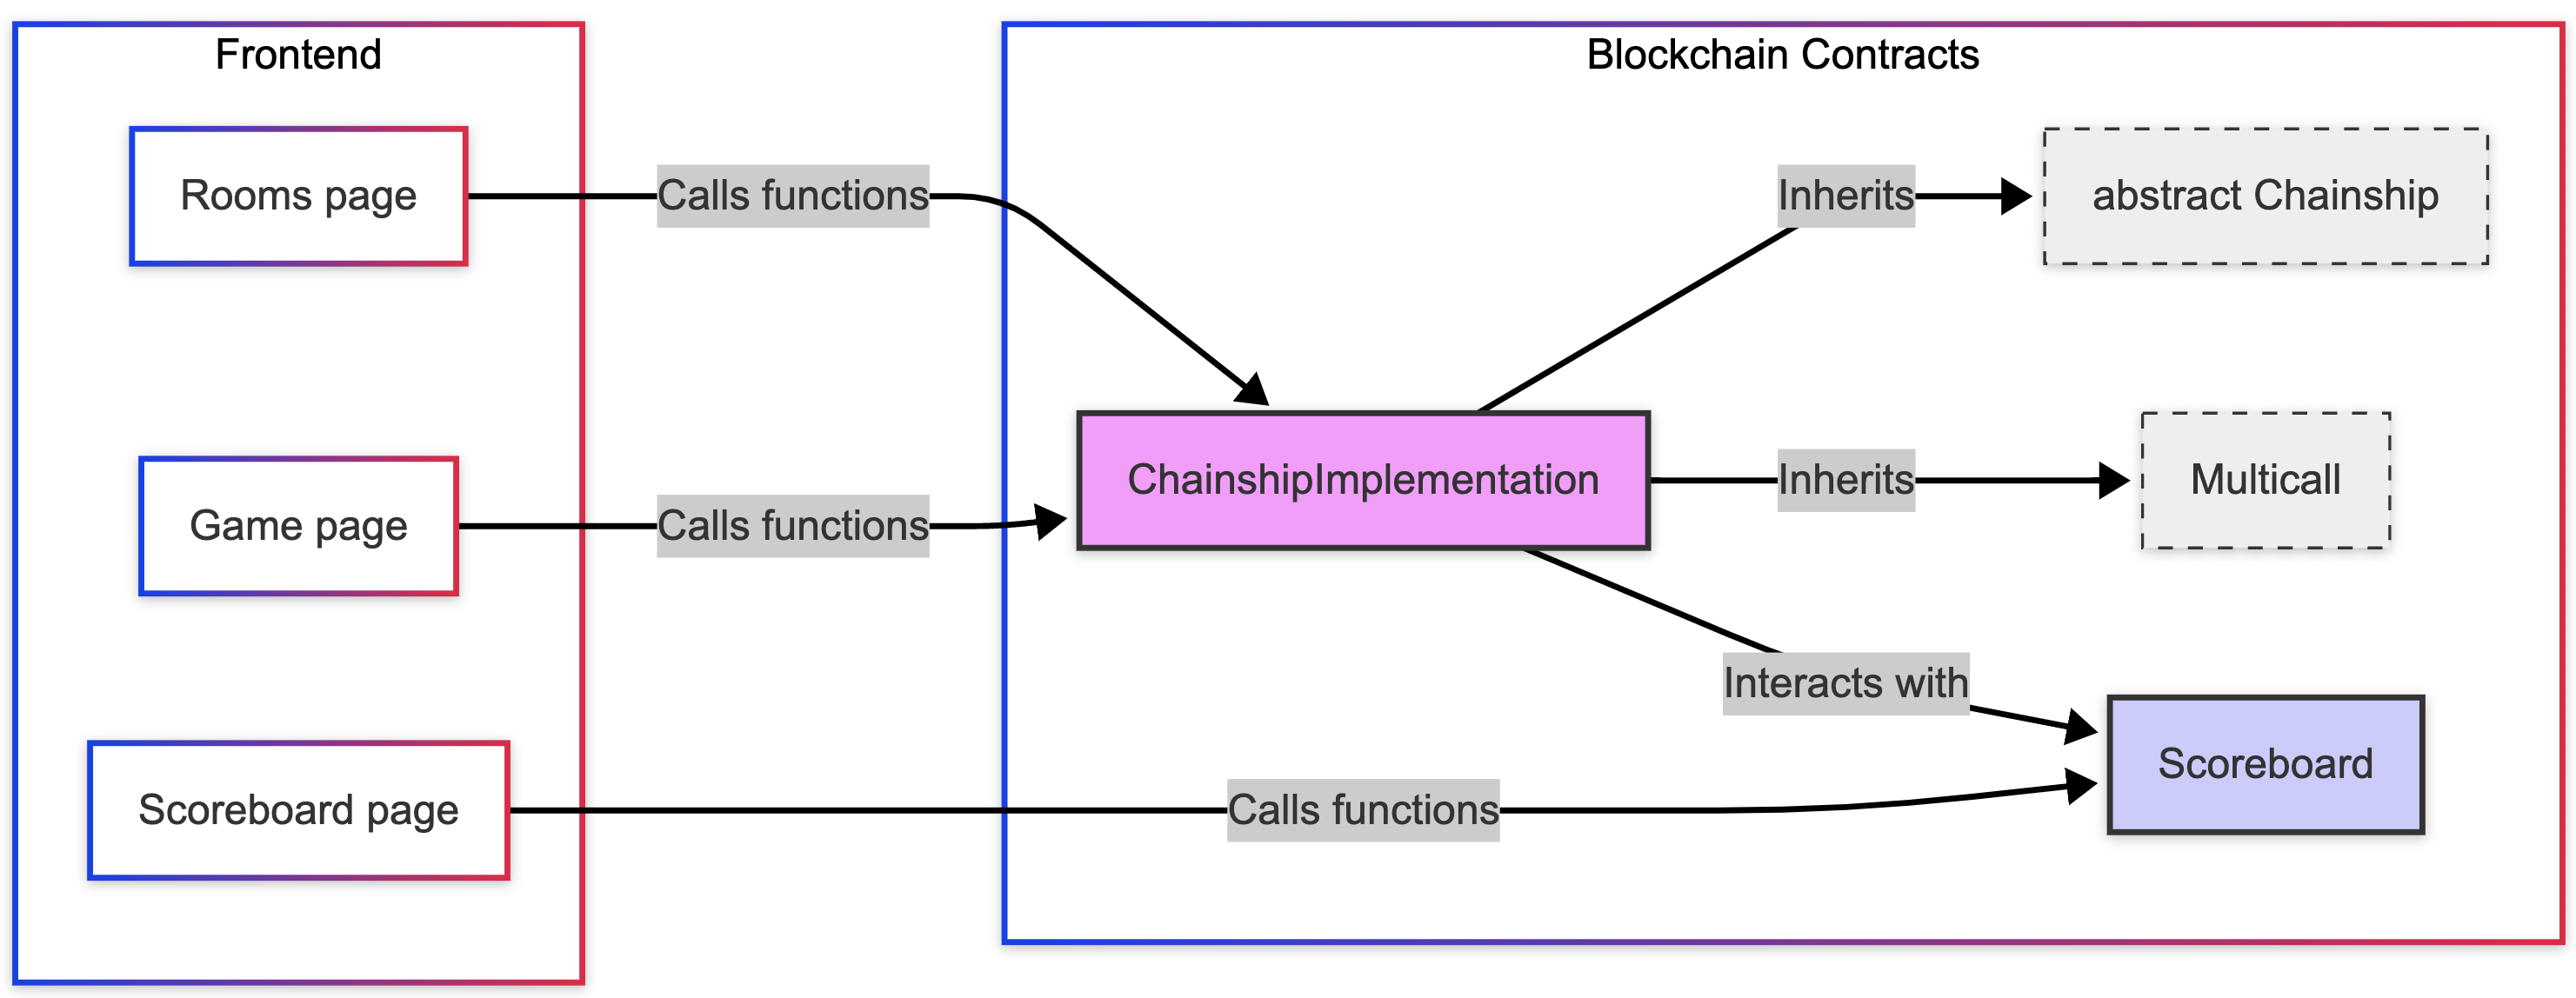
\includegraphics[width=\textwidth]{high-level-architecture.png}
        \caption{High-Level System Architecture}
        \label{fig:architecture}
    \end{figure}

    \subsection{User Interaction Flow}

    A typical game flow involves a sequence of multiple interactions among users, the frontend, Metamask, and the Chainship contract. For simplicity, the diagram below shows only the actions of shooting and answering a shot.

    \begin{figure}[H]
        \noindent\makebox[\textwidth]{%
        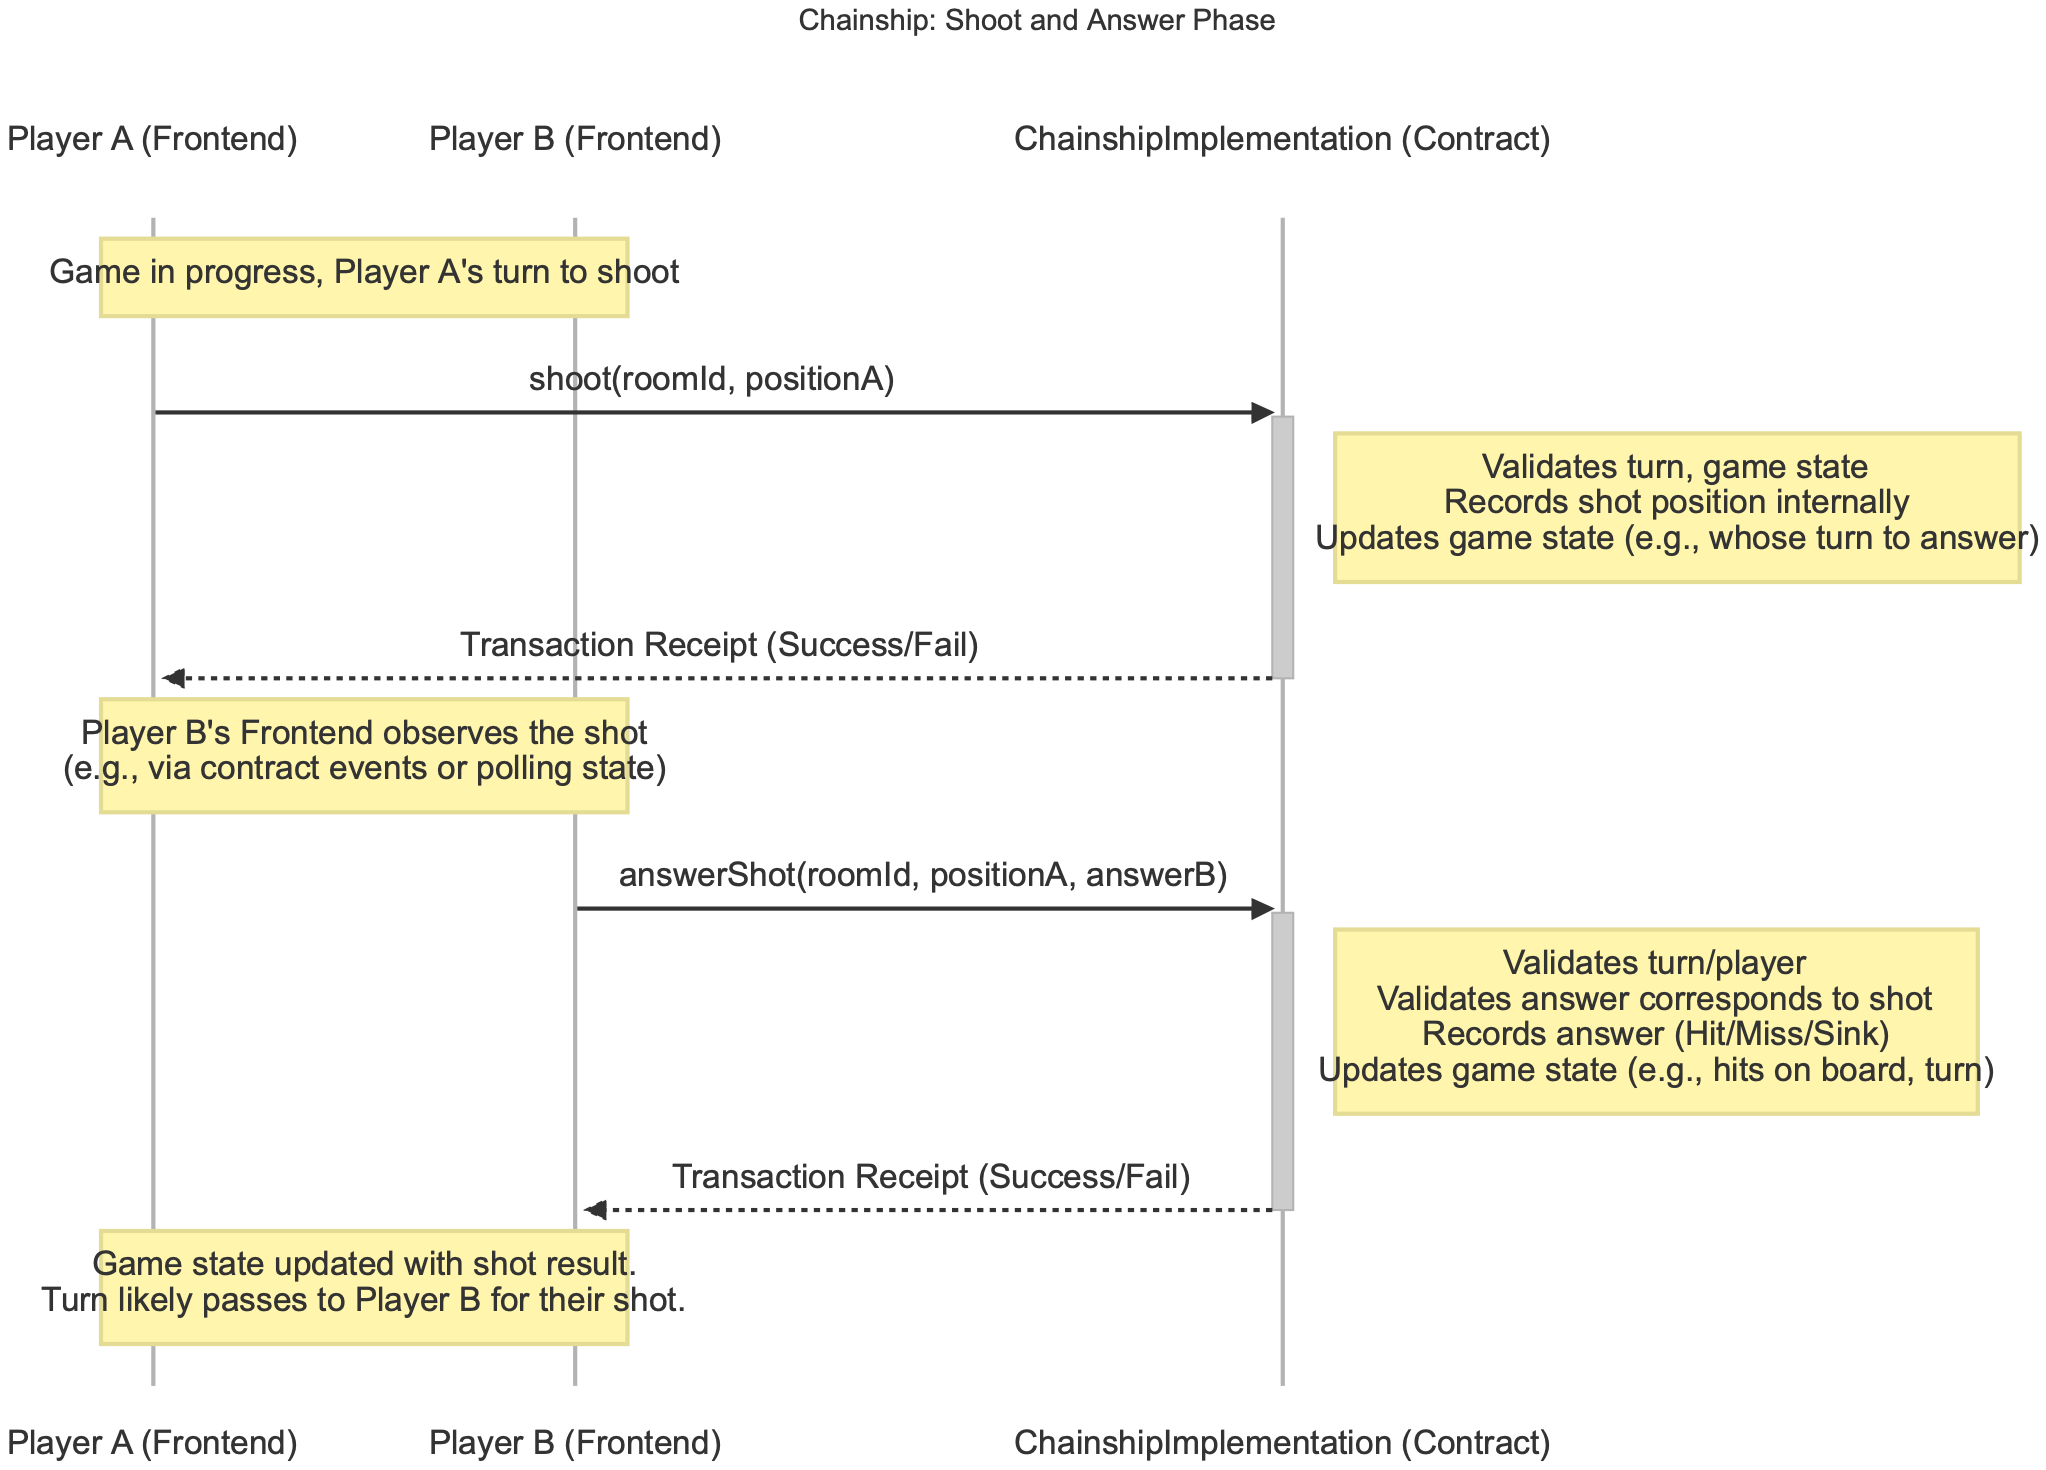
\includegraphics[height=\textwidth, angle=90]{flow.png}}
        \caption{User Interaction Sequence Diagram (Simplified Flow)}
        \label{fig:sequence_diagram}
    \end{figure}

    \section{Smart Contract Design}

    \subsection{Overview}
    The primary contract, \texttt{Chainship}, is abstract and contains the core game logic, state management, and cryptographic verification functions. A concrete implementation, \texttt{Chainship\-Implementation}, inherits from \texttt{Chainship} and provides specific details, such as the commission calculation method. It may optionally inherit from a \texttt{Multicall} contract to enable batching calls for gas efficiency and to reduce delays between player actions, although this is not strictly necessary for the core functionality.

    \subsection{Data Structures}
    Key data structures within the \texttt{Chainship} contract include:
    \begin{itemize}
        \item \texttt{RoomId}: A unique identifier for each game room, derived from a user-provided secret and the contract seed.
        \item \texttt{RoomStatus}: An enum tracking the current stage of the game within a room (e.g., \texttt{Created}, \texttt{Full}, \texttt{Shooting}, \texttt{Finished}).
        \item \texttt{PlayerData}: Stores information for each player, including their address, board commitment hash, number of shots taken, and hashes accumulating their shots and answers.
        \item \texttt{RoomData}: Contains all data for a specific game room, including its status, entry fee, players' data, current turn indicator, and the deadline for the next action.
        \item \texttt{Position}: A struct representing a position on the game board, with x and y coordinates.
        \item \texttt{Answer}: An enum representing the possible answers to a shot (\texttt{Miss}, \texttt{Hit}, \texttt{Sunk}).
        \item \texttt{rooms}: A mapping from \texttt{RoomId} to \texttt{RoomData}, storing the state of all active and past games.
    \end{itemize}

    \subsection{Key Functions}
    The contract provides several functions for player interaction with the game:
    \begin{itemize}
        \item \texttt{createRoom(RoomId, uint256 randomnessCommitment)}: Initializes a new game\break room, setting the entry fee (via \texttt{msg.value}) and registering the creator as Player 1. This function also records Player 1's commitment to their chosen randomness.
        \item \texttt{joinRoom(uint256 roomSecret, uint256 randomnessCommitment)}: Enables a second player to join an existing room. The joining player must provide the correct room secret (which is linked to the \texttt{RoomId}) and match the entry fee. Their commitment to chosen randomness is also recorded.
        \item \texttt{submitBoard(RoomId, uint256 boardCommitment, uint256 randomnesDecommit\-ment)}: Players use this function to submit the commitment of their board layout. They also reveal their previously committed randomness, which is then used to determine the first shooter.
        \item \texttt{shoot(RoomId, Position)}: The player whose turn it is fires a shot at a specified coordinate. This action updates their \texttt{shotsHash}.
        \item \texttt{answerShot(RoomId, Position, Answer)}: The opponent responds to a shot by indicating a \texttt{Miss}, \texttt{Hit}, or \texttt{Sunk}. This updates their \texttt{answersHash}.
        \item \texttt{claimDishonest(RoomId)}: A player can invoke this to accuse their opponent of providing incorrect answers to shots.
        \item \texttt{proveHonesty(RoomId, ...)}: An accused player calls this function to reveal their board layout and complete answer history, aiming to demonstrate they have followed the game rules.
        \item \texttt{proveVictory(RoomId, ...)}: A player initiates this to formally prove they have won the game, typically by demonstrating all opponent's ships have been sunk.
        \item \texttt{claimIdle(RoomId)}: If an opponent fails to act within the specified deadline, a player can call this function to claim victory.
        \item \texttt{receivePrize(RoomId)}: The confirmed winner of a game calls this function to claim the prize pool.
    \end{itemize}

    \subsection{State Machine}
    The game progresses through states defined by the \texttt{RoomStatus} enum. Figure \ref{fig:game_state} illustrates these transitions, which are driven by player actions and enforced by the contract logic (e.g., moving from \texttt{Full} to \texttt{Shooting} only after both players have submitted their boards).

    \subsection{Scoreboard Contract}

    The Scoreboard contract keeps track of the number of points for each player. The Chainship contract calls the Scoreboard contract to update player points. The Scoreboard contract authorizes only specific addresses (i.e., game contracts) to call its update functions. Users can query the number of points for any player.

    Functions provided by the Scoreboard contract:
    \begin{itemize}
        \item \texttt{getPoints(address)}: Returns the number of points for a given player.
        \item \texttt{updateRanking(address player, int256 points)}: Updates the number of points for a given player by adding (or subtracting, if negative) the provided number of points.
        \item \texttt{addGameContract(address)}: Adds a new game contract to the list of authorized game contracts.
        \item \texttt{removeGameContract(address)}: Removes a game contract from the list of authorized game contracts.
    \end{itemize}

    \subsection{External Components}

    The Scoreboard contract inherits from OpenZeppelin's \texttt{Ownable} contract, which is used to restrict access to the \texttt{addGameContract} and \texttt{removeGameContract} functions to the contract owner.

    \subsection{Contracts Diagram}

    The following diagram shows the structure and relationships of the core contracts:

    \begin{figure}[H]
        \noindent\makebox[\textwidth]{%
        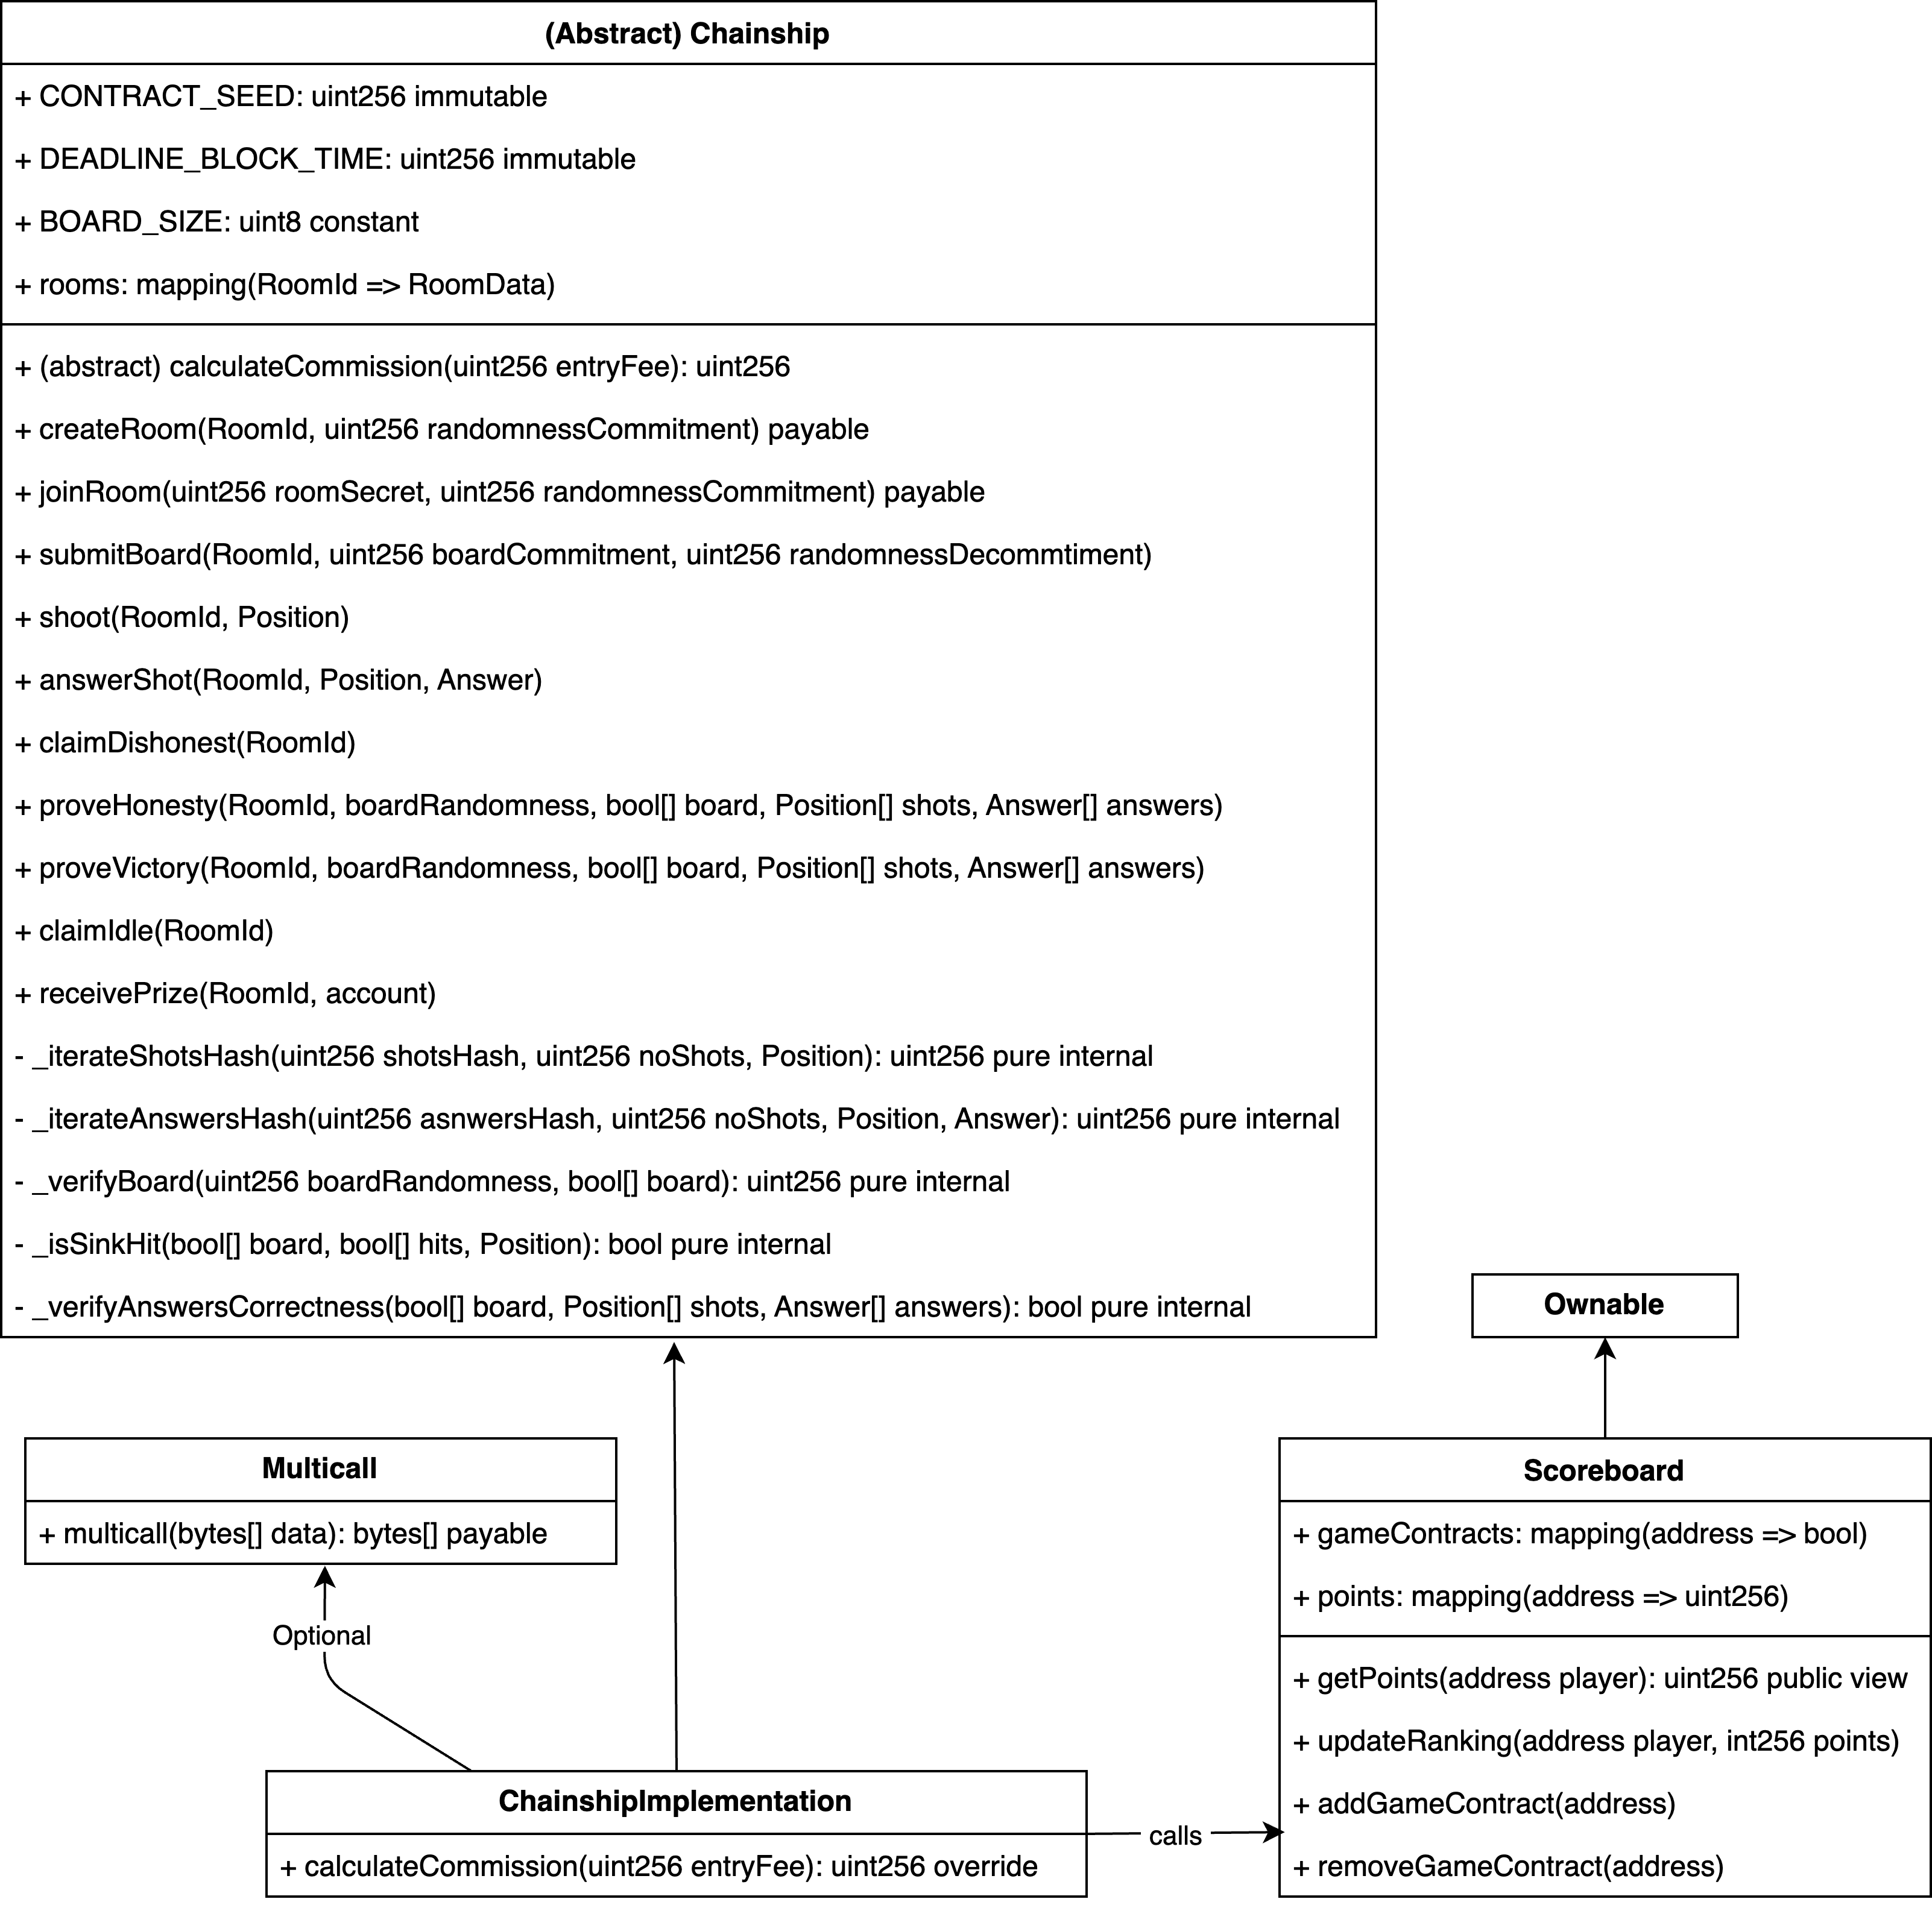
\includegraphics[width=1.25\columnwidth]{uml.png}}
        \caption{Smart Contract UML Class Diagram}
        \label{fig:uml_diagram}
    \end{figure}


    \section{Game Logic}

    \subsection{Game State}

    \begin{figure}[H]
        \centering
        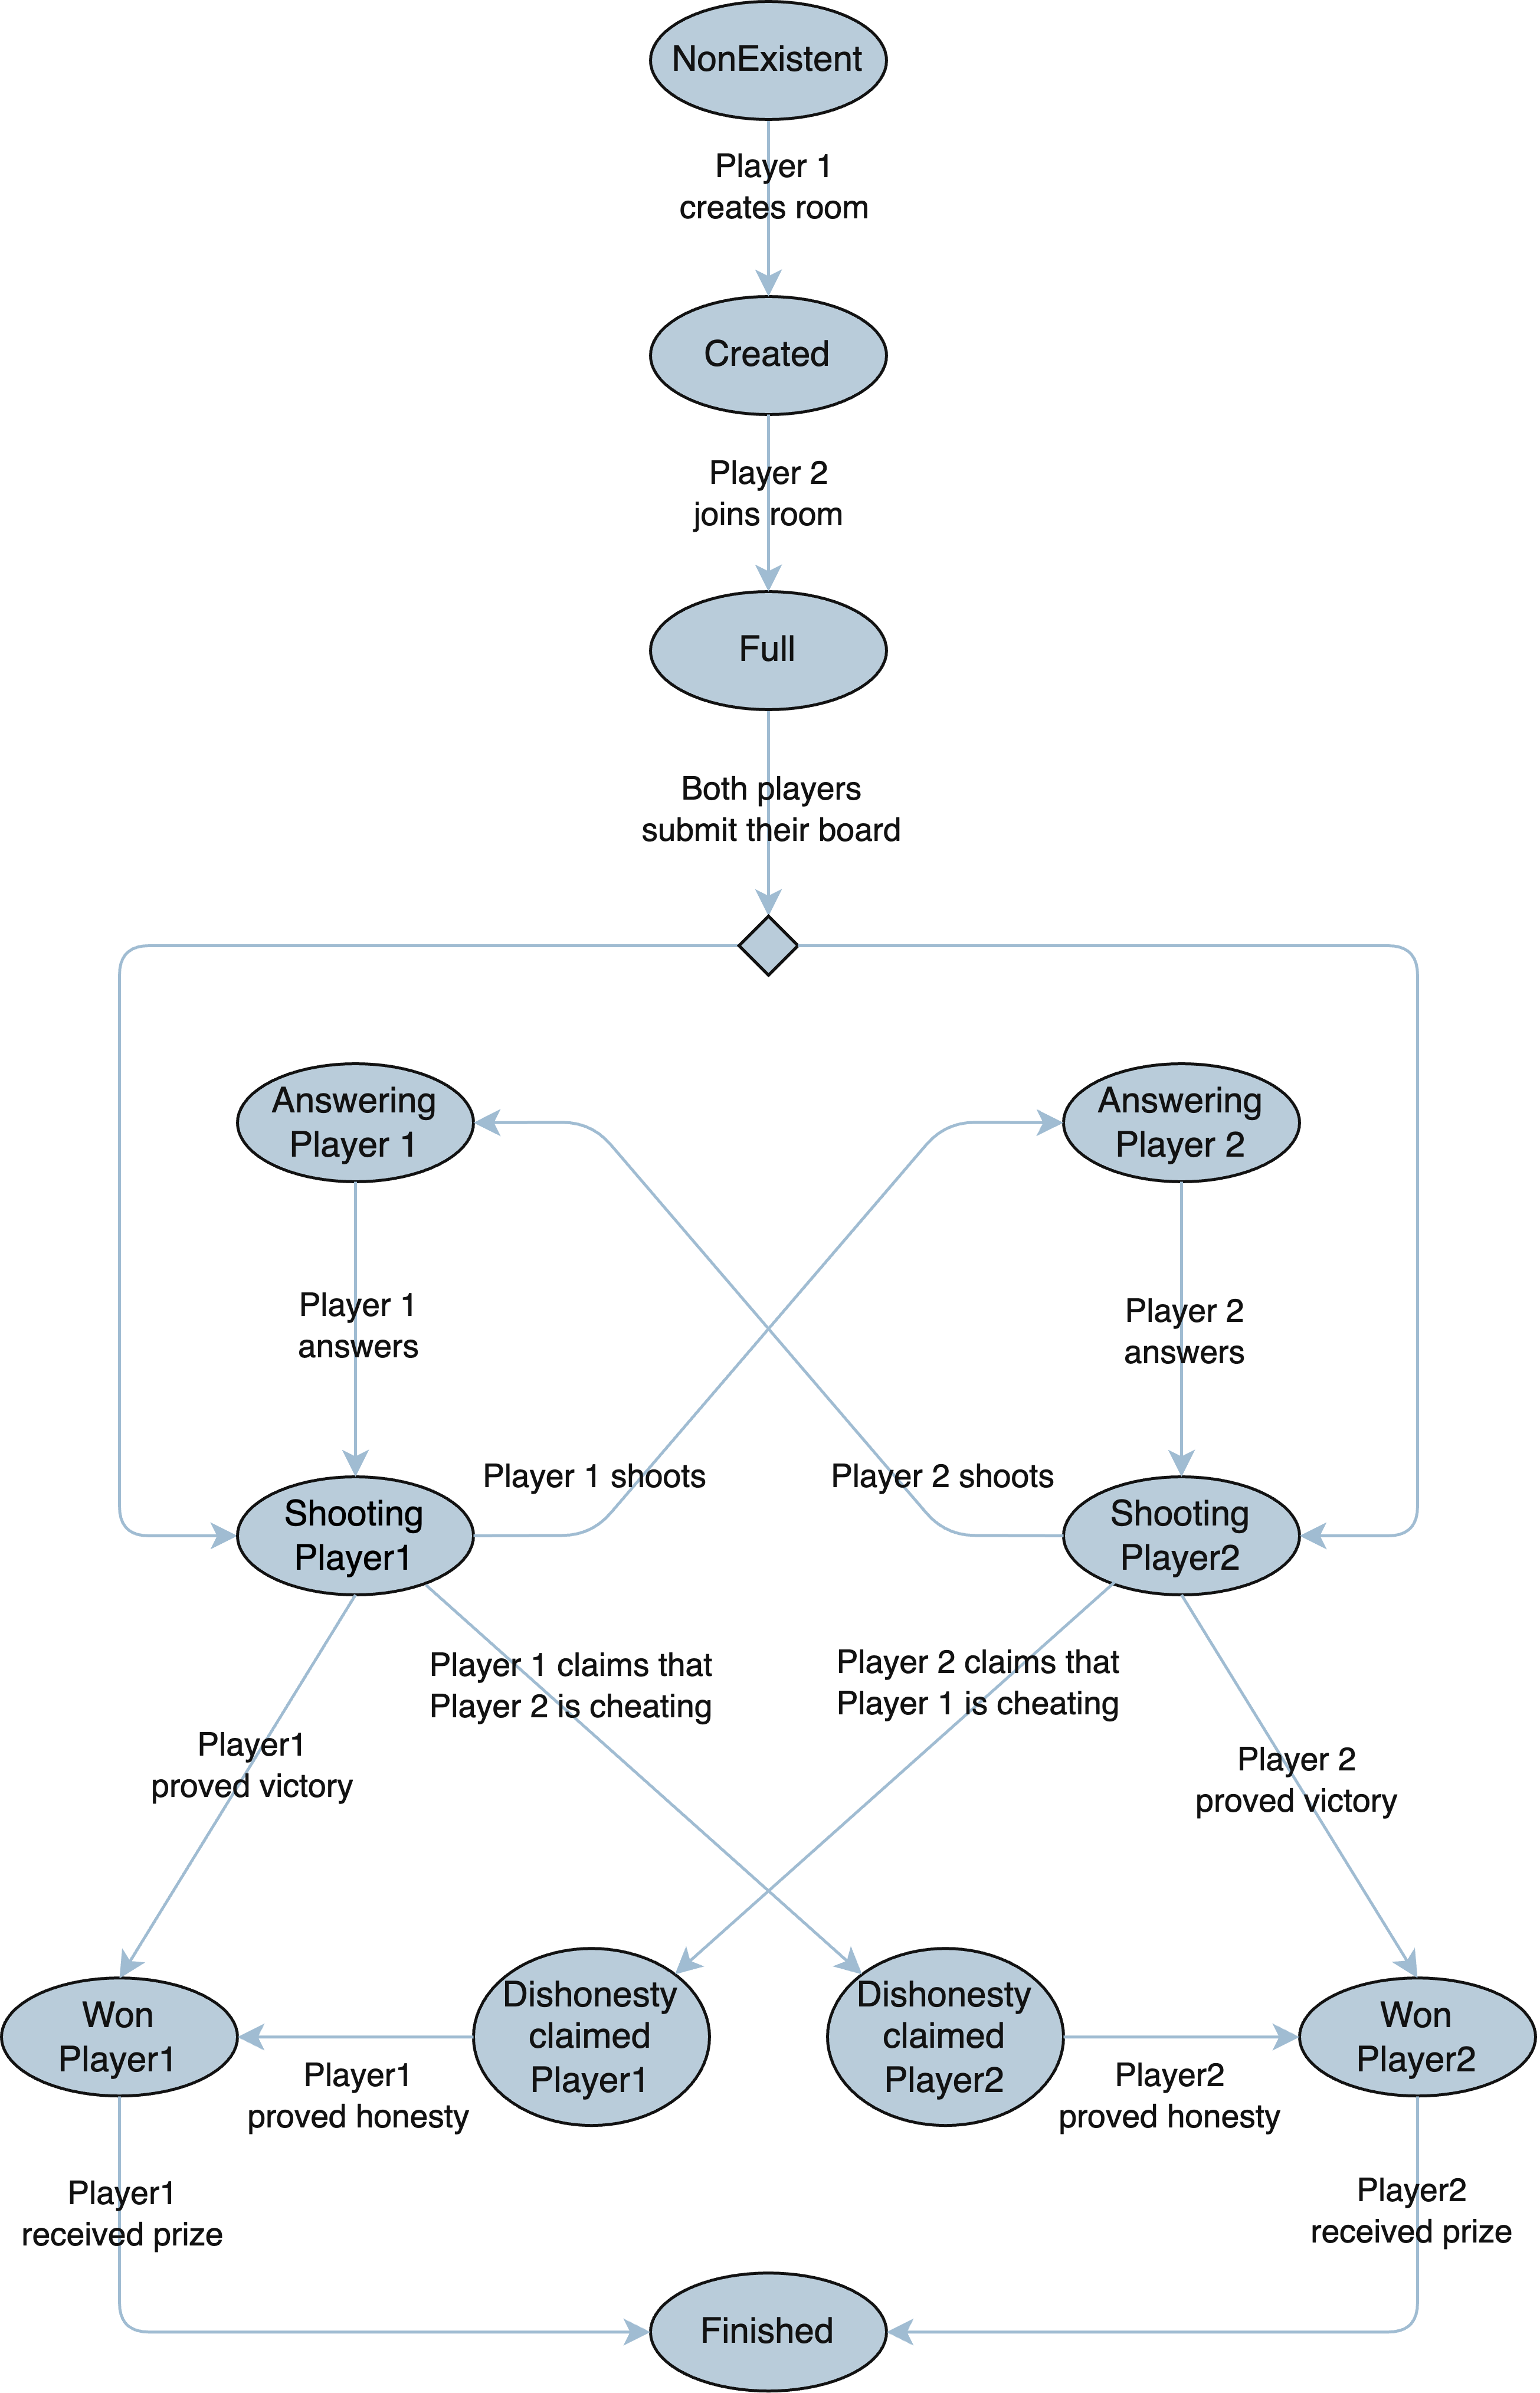
\includegraphics[width=0.8\textwidth]{state.png}
        \caption{Game State Diagram}
        \label{fig:game_state}
    \end{figure}

    \subsection{Randomizing First Shooter}

    Since draws are not allowed, randomizing the first shooter is crucial for fairness. The contract uses a commit-reveal scheme based on player inputs to determine the first shooter. Players commit to their choice of randomness when creating or joining a room. Then, while submitting their boards, they reveal their choices. Both revealed values are combined (e.g., via XOR and modulo operations) to generate a random bit that determines which player starts.

    \subsection{Proof of Victory}

    Players can win in several ways:
    \begin{enumerate}
        \item \textbf{Sinking all enemy ships:} This requires the winning player to prove that their shots correctly led to sinking all opponent's ships, consistent with the opponent's answers (and potentially revealed board if dishonesty was claimed).
        \item \textbf{Opponent Dishonesty:} A player can claim their opponent answered incorrectly using \texttt{claimDishonest}. If the accused opponent fails to prove their honesty via \texttt{proveHonesty} within the stipulated deadline, the accuser wins.
        \item \textbf{Opponent Idleness:} If an opponent fails to perform a required action (such as \texttt{submitBoard}, \texttt{shoot}, \texttt{answerShot}, or \texttt{proveHonesty}) before the \texttt{answerDeadline}, the other player can claim victory.
    \end{enumerate}
    In all cases, after the winner is determined, they must call the \texttt{receivePrize} function to claim their winnings.
    
    To prove honesty after a \texttt{claimDishonest} call, the accused player invokes \texttt{proveHonesty}, providing their board's salt (\texttt{boardRandomness}), the board layout (\texttt{board}), the sequence of shots they received (\texttt{shots}), and the answers they gave (\texttt{answers}). The contract then verifies:
    \begin{enumerate}
        \item \textbf{Board Commitment:} That \texttt{\_verifyBoard(boardRandomness, board)} matches the stored \texttt{boardCommitment}.
        \item \textbf{Shot History:} That the provided \texttt{shots} sequence hashes to the opponent's stored \texttt{shotsHash}.
        \item \textbf{Answer History:} That the provided \texttt{answers} sequence (along with \texttt{shots}) hashes to the accused player's stored \texttt{answersHash}.
        \item \textbf{Answer Correctness:} That \texttt{\_verifyAnswerCorrectness} confirms each answer in \texttt{answers} was correct given the \texttt{board} and the sequence of \texttt{shots}.
    \end{enumerate}

    To prove victory by sinking all ships, the winner calls \texttt{proveVictory}. This involves providing arguments that are the same as those in \texttt{proveHonesty}, along with answers received from the opponent. This allows the contract to verify that all the opponent's ships were sunk according to the game rules.

    \section{Cryptography}

    \subsection{Board Commitment}
    To prevent players from changing their ship layout mid-game and to hide it from their opponent, a commitment scheme is utilized. A player commits to their board \( b \) (represented as a flat \texttt{bool[BOARD\_SIZE*BOARD\_SIZE]} array) combined with a secret random salt \( r \) (\texttt{boardRandomness}).

    \[ \operatorname{BoardCommitment}(b, r) = \operatorname{keccak256}(\text{abi.encodePacked}(r, b)) \]

    The salt \( r \) prevents pre-image attacks where an opponent might pre-calculate commitments for all possible valid boards, especially if the board size were small. The player reveals \( b \) and \( r \) only when required (e.g., during a \texttt{proveHonesty} call). The internal \texttt{\_verifyBoard} function also checks the validity of the board layout itself (e.g., ensuring ships do not touch diagonally and adhere to correct sizes).

    \subsection{Shots Hash}

    To efficiently verify the sequence of shots taken by a player without storing each shot individually on-chain, an iterative hashing approach is employed. Let \( h_0 = 0 \). For the \( i \)-th shot at position \( (x_i, y_i) \), the hash \( h_i \) is calculated based on the previous hash \( h_{i-1} \), the shot number \( i \), and the coordinates:

    \[ h_i = \operatorname{keccak256}(\text{abi.encodePacked}(h_{i-1}, i, x_i, y_i)) \quad \text{for } i = 1, 2, \ldots, n \]

    The final hash \( h_n \) (stored as \texttt{shotsHash}) represents the entire sequence of \( n \) shots. This design allows the contract to store only the latest hash and the shot count (\texttt{noShots}). Verification involves the challenged player providing the full sequence of shots, which is then re-hashed iteratively by the contract to check if it matches the stored final hash.

    \subsection{Answers Hash}

    Similarly, an iterative hash (stored as \texttt{answersHash}) accumulates the answers given by a player. For the \( i \)-th shot received at \( (x_i, y_i) \) with answer \( a_i \) (an \texttt{Answer} enum value), the hash is updated:

    \[ h'_i = \operatorname{keccak256}(\text{abi.encodePacked}(h'_{i-1}, i, x_i, y_i, a_i)) \quad \text{for } i = 1, 2, \ldots, n \]

    where \( h'_0 = 0 \). This enables verification of the entire answer sequence during the \texttt{proveHonesty} phase by comparing the recomputed hash with the stored \texttt{answersHash}.

    \subsection{Commit-Reveal for Randomness}

    To fairly establish the starting player, a Commit-Reveal scheme is employed. Both players, \(P_1\) and \(P_2\), first commit to a secret nonce \(N_i\) by submitting its cryptographic hash \(C_i = \operatorname{keccak256}(N_i)\) to the smart contract:
    \[C_1 = \operatorname{keccak256}(N_1)\]
    \[C_2 = \operatorname{keccak256}(N_2)\]
    Once both commitments are recorded on-chain, players reveal their nonces \(N_1\) and \(N_2\). The contract verifies these revealed nonces against the previously stored commitments. A shared random value \(R\) is then derived from the revealed nonces, for instance, by XORing them and taking the result modulo 2 to select the starting player:
    \[R = (N_1 \oplus N_2) \pmod 2\]
    This mechanism prevents either player from unfairly influencing the outcome after observing the other's commitment.

    \section{Estimations}
    
    \subsection{Unit Tests}
    Unit tests will verify the correct behavior of individual functions in isolation.

    \begin{itemize}
        \item \textbf{\texttt{Chainship} Contract:}
        \begin{itemize}
            \item \texttt{constructor}: \(\approx\) 1 test case (initial state, immutable variables).
            \item \texttt{roomSecretToId}: \(\approx\) 2 test cases (correct ID generation, different secrets yield different IDs).
            \item \texttt{createRoom}: \(\approx\) 4 test cases (success, entry fee less than/equal to commission, room already exists, event emission).
            \item \texttt{joinRoom}: \(\approx\) 5 test cases (success, room not in correct state, entry fee mismatch, event emission, deadline setting).
            \item \texttt{\_getPlayerNumber} (internal): \(\approx\) 3 test cases (player 0, player 1, not a player).
            \item \texttt{submitBoard}: \(\approx\) 7 test cases (success P1 then P2, board commitment zero, wrong room state, past deadline, non-player sender, already submitted, event emissions).
            \item \texttt{\_iterateShotsHash} (internal): \(\approx\) 3 test cases (valid position, invalid position, correct hash).
            \item \texttt{shoot}: \(\approx\) 6 test cases (success, wrong room state, not player's turn, invalid position, state changes, event emission).
            \item \texttt{\_iterateAnswersHash} (internal): \(\approx\) 3 test cases (valid position/answer, invalid position, correct hash).
            \item \texttt{answerShot}: \(\approx\) 6 test cases (success, wrong room state, non-player sender, invalid position, state changes, event emission).
            \item \texttt{claimDishonest}: \(\approx\) 5 test cases (success, wrong room state, non-player sender, state changes, event emission).
            \item \texttt{\_verifyBoard} (internal): \(\approx\) 4+ test cases (valid board, invalid size, various invalid ship placements, correct commitment).
            \item \texttt{\_isSinkHit} (internal): \(\approx\) 4+ test cases (not hit, hit not sink, hit and sink, edge cases).
            \item \texttt{\_verifyAnswerCorrectness} (internal): \(\approx\) 4+ test cases (correct sequence, length mismatch, various incorrect answer scenarios, hash/hit count correctness).
            \item \texttt{proveHonesty}: \(\approx\) 9 test cases (success, wrong room state, not accused player's turn, board commitment mismatch, shots hash mismatch, answers hash mismatch, incorrect answer position, state changes, event emission).
            \item \texttt{claimIdle}: \(\approx\) 4 test cases (successful claim for opponent not submitting board, successful claim for opponent not acting in turn, deadline not passed, wrong state).
            \item \texttt{receivePrize}: \(\approx\) 5 test cases (success, not winner, game not finished, fund transfer, reverting receive function).
            \item First-player randomization (commit-reveal): \(\approx\) 3 test cases (valid and invalid commitments, correct determination).
        \end{itemize}
        Estimated unit tests for \texttt{Chainship}: \textbf{\(\approx\) 78+}.

        \item \textbf{\texttt{Scoreboard} Contract:}
        \begin{itemize}
            \item \texttt{getPoints}: \(\approx\) 2 test cases (player exists/does not exist).
            \item \texttt{updateRanking}: \(\approx\) 3 test cases (success add/subtract points, unauthorized call by non-game contract).
            \item \texttt{addGameContract}: \(\approx\) 2 test cases (success by owner, failure by non-owner).
            \item \texttt{removeGameContract}: \(\approx\) 2 test cases (success by owner, failure by non-owner).
        \end{itemize}
        Estimated unit tests for \texttt{Scoreboard}: \textbf{\(\approx\) 9}.
    \end{itemize}
    \textbf{Total estimated unit tests: \(\approx\) 86+}.

    \subsection{Integration Tests}
    Integration tests will verify the interaction between functions and contracts across key user scenarios.
    \begin{itemize}
        \item \textbf{Scenario 1: Full Game Flow:}
        Player 1 creates a room. Player 2 joins. Both players submit boards. Players exchange several shots and answers correctly. Simulate a scenario leading to standard win by proving victory.
        \item \textbf{Scenario 2: Dishonesty Claim:}
        Game setup as above. Player A makes an intentionally incorrect answer. Player B calls \texttt{claimDishonest}.
        \begin{itemize}
            \item Path 2a: Player A successfully calls \texttt{proveHonesty} with correct data, opponent (Player B) loses.
            \item Path 2b: Player A provides inconsistent data to \texttt{proveHonesty}, call reverts or honesty is not proven, Player B wins.
        \end{itemize}
        \item \textbf{Scenario 3: Game End due to Idleness:}
        \begin{itemize}
            \item Path 3a (Board Submission): Player 2 joins but fails to submit their board within the deadline. Player 1 calls \texttt{claimIdle} and wins.
            \item Path 3b (Shooting/Answering): During the game, the active player fails to \texttt{shoot} or \texttt{answerShot} within the deadline. The other player calls \texttt{claimIdle} and wins.
            \item Path 3c (Prove Honesty): After a \texttt{claimDishonest}, the accused player fails to call \texttt{proveHonesty} within the deadline. The accuser calls \texttt{claimIdle} and wins.
        \end{itemize}
        \item \textbf{Scenario 4: Scoreboard Interaction:}
        After a game concludes (e.g., via scenarios above), verify that if the \texttt{Scoreboard} contract were integrated, the \texttt{Chainship} contract would correctly call \texttt{updateRanking} on the \texttt{Scoreboard}.
        \item \textbf{Scenario 5: First-Player Randomization:}
        Test the commit-reveal scheme for determining the first player, covering various inputs and ensuring fairness.
        \item \textbf{Scenario 6: Prize Distribution:}
        Test the correct distribution of the prize pool to the winner and commission handling.
    \end{itemize}

    \subsection{Implementation Time Estimation}
    To estimate the project implementation time for smart contract development, a method based on the number of key operations and the number of involved contracts is used.

    \begin{itemize}
        \item \textbf{\texttt{Chainship} Contract:}
        Key operations:
        \begin{itemize}
            \item \texttt{createRoom}
            \item \texttt{joinRoom}
            \item \texttt{submitBoard}
            \item \texttt{shoot}
            \item \texttt{answerShot}
            \item \texttt{claimDishonest}
            \item \texttt{proveHonesty}
            \item \texttt{proveVictory}
            \item \texttt{claimIdle}
            \item \texttt{receivePrize}
        \end{itemize}
        Total key operations for \texttt{Chainship}: \(L_{op1} = 10\).

        \item \textbf{\texttt{Scoreboard} Contract:}
        Key operations:
        \begin{itemize}
            \item \texttt{updateRanking}
            \item \texttt{addGameContract}
            \item \texttt{removeGameContract}
            \item \texttt{getPoints}
        \end{itemize}
        Total key operations for \texttt{Scoreboard}: \(L_{op2} = 4\).
    \end{itemize}

    Total number of key operations \( L_{op} = L_{op1} + L_{op2} = 10 + 4 = 14 \).
    Number of main contracts to implement\( L_k = 2 \) (\texttt{Chainship} and \texttt{Scoreboard}).

    Estimated project complexity factor \( W = L_{op} \times L_k = 14 \times 2 = 28 \) units.
    
    Assuming that in one day one can work on 2 units, the project will take 14 days to complete.

    \section{Summary}

    The Chainship project aims to deliver a decentralized Battleship game on EVM-compatible blockchains, emphasizing security, transparency, and fairness. The core of the system is the \texttt{Chainship} smart contract, which manages all aspects of game creation, progression, and fund distribution, eliminating the need for a central authority. A secondary \texttt{Scoreboard} contract provides a persistent ranking system.

    Key architectural features include:
    \begin{itemize}
        \item \textbf{Decentralized Game Logic:} All game rules and state transitions are enforced by the smart contract.
        \item \textbf{Cryptographic Commitments:} \texttt{keccak256}-based commitment schemes are used for board placements and first-player randomization, preventing cheating and ensuring hidden information until reveal.
        \item \textbf{Iterative Hashing:} Sequences of shots and answers are hashed iteratively to save storage and gas costs, while still allowing for on-chain verification.
        \item \textbf{Player-Driven Dispute Resolution:} Mechanisms like \texttt{claimDishonest} and \texttt{proveHonesty} allow players to resolve disputes on-chain.
        \item \textbf{Modularity:} The system is designed with a main game contract (\texttt{Chainship}) and a separate \texttt{Scoreboard} contract, potentially allowing for future expansion or integration with other games.
        \item \textbf{Frontend Interaction:} A web-based frontend application will enable user interaction with the game via wallets like Metamask.
    \end{itemize}
    The project leverages Solidity for smart contract development and standard cryptographic techniques to build a robust and trustworthy gaming platform. The architecture is designed to minimize trust assumptions and provide a verifiable gaming experience.

\end{document}
